\section{多次反射与当前实际}
\label{sec:5.5}

返地表处有种种未固结物质,诸如水、土壤以及所谓风化带等,这些近地表物质与下面
的石油储集岩层之间的波阻抗差异往往甚为显著,足以产生形形色色的近地表谐振,这些谐
振现象是无法预测的,而且不能用前面几章所述的方法加以解释。

\subsection{硬海底例子}
\label{sec:5.5.1}

图\ref{fig:mltp/multiple}所示是质量极佳的海底多次反射,各双曲线$v^2t^2-x^2
=z_j^2$按均勻间隔$z_j=j\Delta z$出
现,$j=0,1,2......$。除球面发散校正以外,数据未经任何处理。空气比水轻、速度比水层速
度慢,而海底沉积则儿乎总是比水层致密些和速度快一些,这意味着相继出现的多次反射差
不多总是具有交替变化的极性。地震初至的极性通常是模棱两可的,但是此图却波形清晰而
且逐个反射极性交替变化明显可见。相继到达之多次反射的振幅比就是反射系数,图\ref{fig:mltp/multiple}
中的反射系数看来是-0.7左右。多次反射首波(multiply reflected head wave)也
较明显,极性也是一样地交错改变。由于首波的多次反射出现在临界角,它们应具有反射系数
-1.0。我们可见到它们实际是逐级增强的,之所以增强其原因就在于球面扩散校正是以三维传播为基础,
而首波实际是作二维传播的。

就波动理论来说,多次反射是有趣的现象,但是对于地球物理学家,它们却是种严重障
碍,地球物理学家不喜欢见到的携带信息的一次波被多次反射掩盖了。



\begin{figure}[H]
\centering
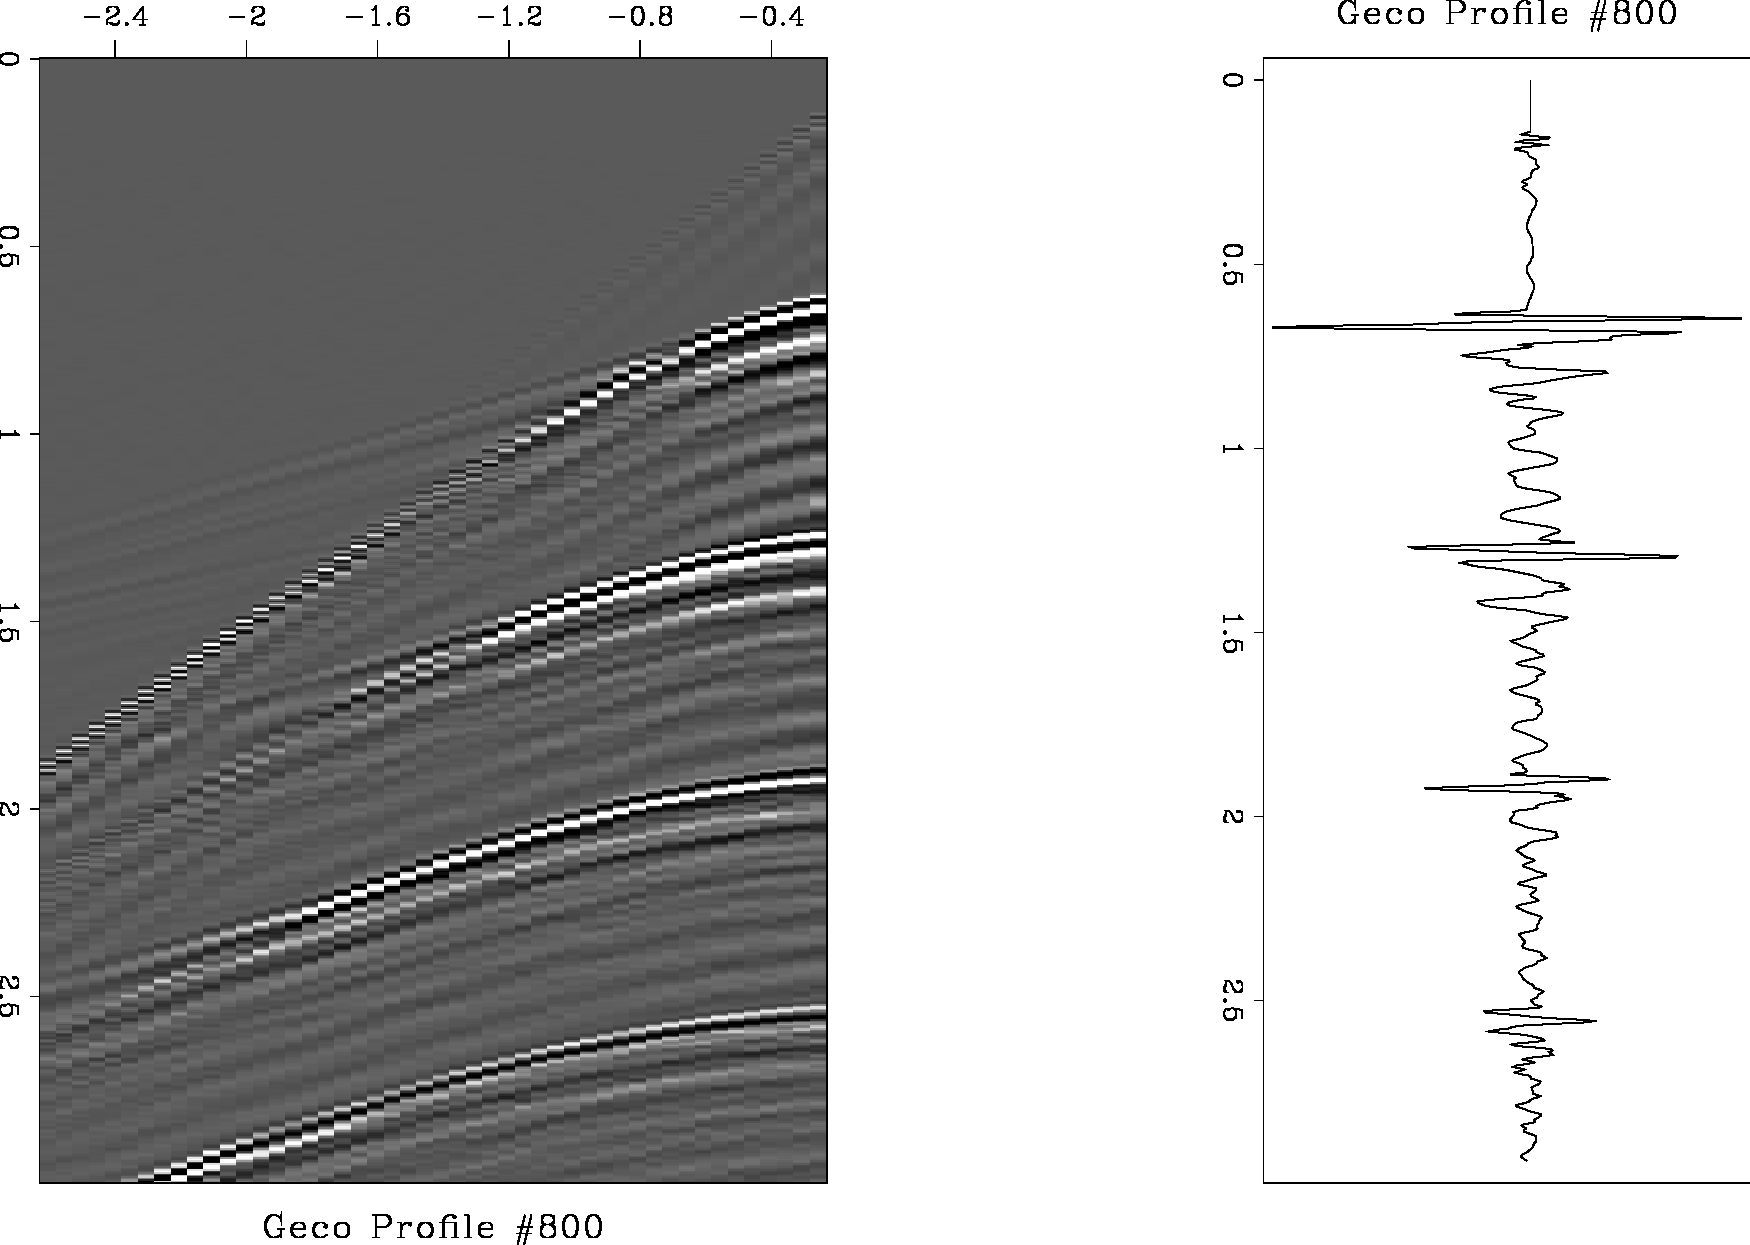
\includegraphics[width=0.65\textwidth]{mltp/multiple}
\caption[multiple]{挪威的多次反射海上剖面。左侧是经过放大的近炮点记录道(据挪威GECO公司)
}
\label{fig:mltp/multiple}
\end{figure}

\subsection{常规数据处理中的反褶积}
\label{sec:5.5.2}

在图\ref{fig:mltp/multiple}中,海水层深度比典型石油勘探深度要大些,图\ref{fig:mltp/gsidecon}与图\ref{fig:mltp/pns}才是更典型的情形。在图\ref{fig:mltp/gsidecon}中,海水层深度浅到不可能辨别出反射了。就陆地资料来说,风化层底部
通常很浅且模糊不清,以致一般不可能识别出单独的反射。“浅”这个字眼R用于多次反射
时是限定只指反射记录变化很迅速,以至没办法钯它们彼此明显区别开来。

\begin{figure}[H]
\centering
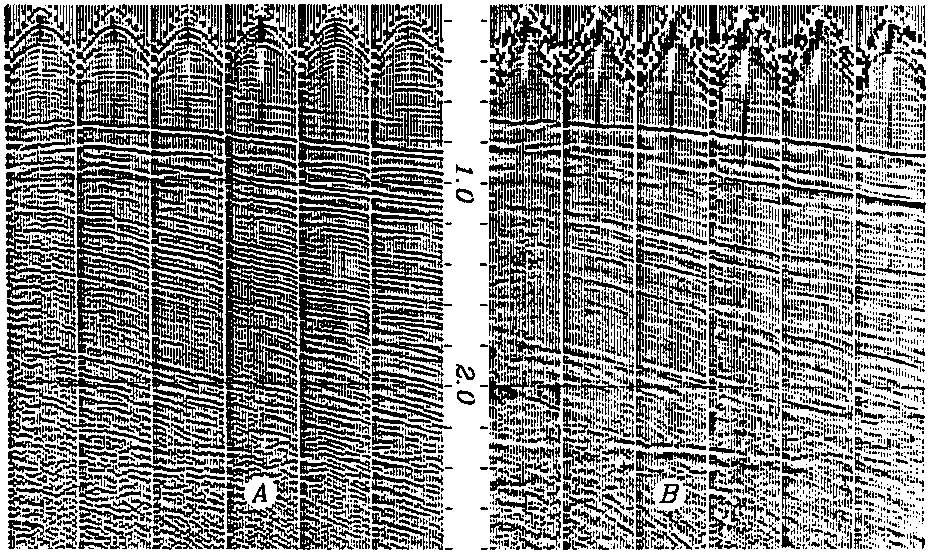
\includegraphics[width=0.65\textwidth]{mltp/gsidecon}
\caption[gsidecon]{
反褶积之前(左图)和反褶积之后(右图)的野外剖面(GSI公司公布,
公元1965年)
}
\label{fig:mltp/gsidecon}
\end{figure}

\begin{figure}[H]
\centering
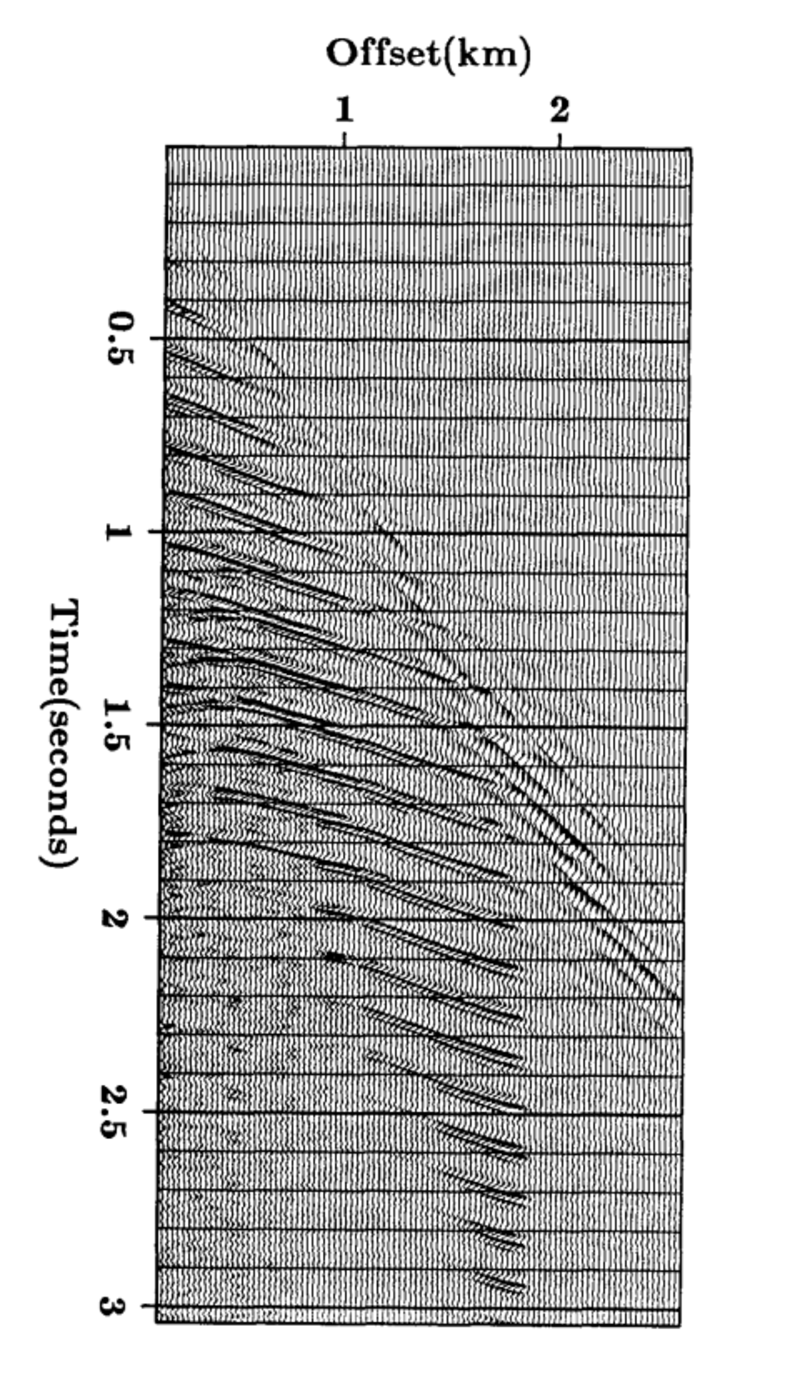
\includegraphics[width=0.65\textwidth]{mltp/pns}
\caption[pns]{
北海剖面(西方地球物理公司)。具有周期大约为90毫秒
之很强的交混回响,它们是海底的多次反射。注意,最强
的信号出现在随时间增长而增大的炮检距上,这是因为最强
的多次波常常在临界角上出现。在船后1.8公里处交混回响
强度突然减低,这是暗示在该点处的海底有突然变化。
}
\label{fig:mltp/pns}
\end{figure}

关于反褶积这个题目,统计学家已经写了一大堆丰富文献了,对于他们来说,这问题实际
是一个估计震源波形而不是消除多次反射的问题。在一定的数学极限之内可使震源波形问題
等价于多次反射问题,当混响只限于炮点或
检波点周围很小的物理体积之内、诸如在土壤
层之内时,这种极限就能成立。震源波形与多
次反射问题之所以能够在这神情形下等价,原
因就在于炮点产生的下行波不但对于炮点本身
来说是固有的,而且也包括了局部土壤层的共
振。在反射地震学中,虚反射这个词是指震源
的反射再加上来自地面的反射(或有时来自风
化层底部),因为震源非常接近这些反射面,
所以我们往往把虚反射也看成是震源波形的一部分。

关于垂直入射情形下的多次反射模型,也
有广泛的文献。在波动传播理论工作者当中,
把消除多次波称作反演问题。看起来,要使反
演理论能应用于实际问题。必须同可处理爆烊
波形未知、频谱性质欠缺问题的分析方法结合起来才行。

常规生产性的反褶积(图\ref{fig:mltp/gsidecon})有许多
种导忠方法积解释,我将以简单的术语来阐述
那些我相信是反褶积之本质的一些问题。每个
地震记录都有一个谱,该谱是许多因素产生的
结果,某些因素具有基本意义,另一些兜j是不增大的炮检距上,这是因为最强的多次波常常在临界角上
重要的。当迆震记录正好因某种近地表现象而
产生共鸣震荡时,这就使人感到麻烦了。反褶积
基本上是这么一种处理:测定出强共鸣震荡,然后设计一种滤波处理去皮制它们。所设
计的滤波具有一种特定的谱,它应大致等于原始数据之谱的倒数,因而,滤波的输出大致为
白噪(所有频率成分均相等)。从最早期开始,地震学家就已经发现反射地震数据在10至
100赫兹频带之外很少有多大意义,所以采取的最后一个步骤就是将该频带范围之外的频率
成分均消除。(对大多数地震学家来说,关于输出的谱应为白噪的假设看来是一稗不得已的
假设,但是实践通常都表明,比起从原始数据来解释地层映象,那它还是更可取的)。

% \begin{figure}[H]
% \centering
% 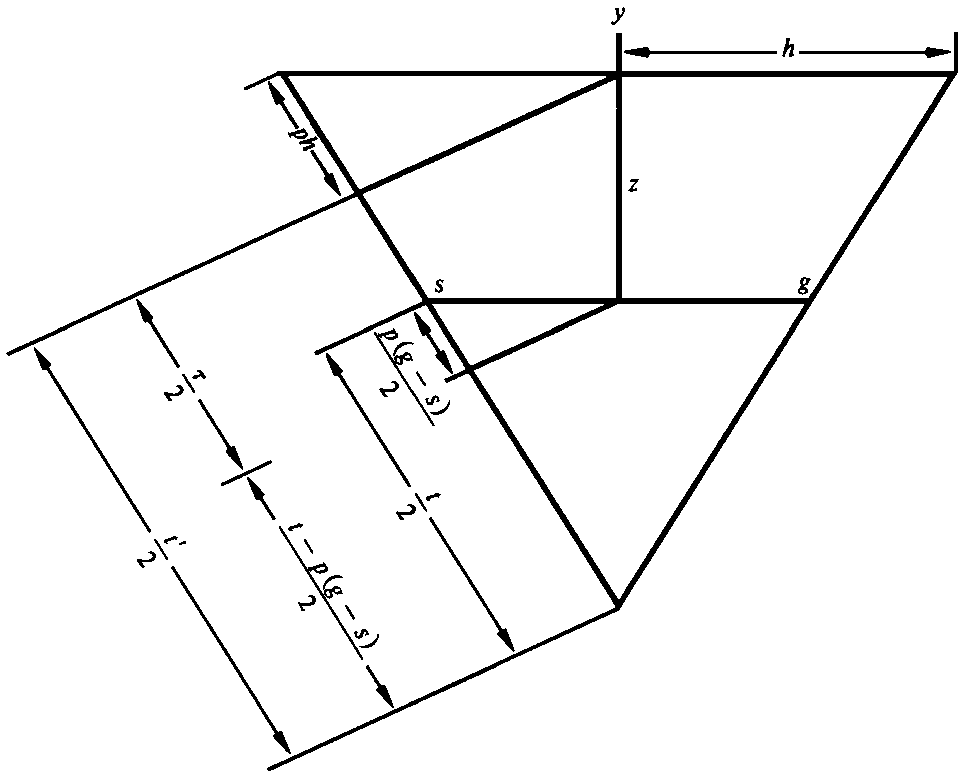
\includegraphics[width=0.65\textwidth]{slnt/cmplmo}
% \caption[cmplmo]{共中心点道集与LMO时间坐标框架几何形态,对于描迷类似于一种参考Snell
% 的各种波场,这是一种很自然的坐标系统
% }
% \label{fig:slnt/cmplmo}
% \end{figure}

% 由图\ref{fig:slnt/cmplmo}所示几何关系将得出结论:观测某个特定值$(h',t')$时的反射,直接就可确定
% 速度。反射面深度之方程可写出为
% \begin{equation}
% \text{反射面深度}=\frac{h'}{\tah\theta}=v(\frac{t'}{2}+ph')\cos\theta
% \label{eq:ex5.4.18}
% \end{equation}

% 利用Snell定律消去其中的角度,然后解出速度,得
% \begin{equation}
% v^2=\frac{1}{p}\frac{1}{p+\frac{t'}{2h'}}
% \label{eq:ex5.4.19}
% \end{equation}
% 此式同式\ref{eq:ex5.4.12}完全一致。

% 将上述各项定义集中为一组方程,并以遍及z的积分来代替z以便允许速度随
% 深度而变化,我们得出:
% \begin{subequations}
% \begin{equation}
% t'(t,g,s,z)=t-(g-s)+2\int_0^z\frac{\cos\theta}{v}dz
% \label{eq:ex5.4.20a}
% \end{equation}
% \begin{equation}
% y(t,g,s,z)=\frac{g+s}{2}
% \label{eq:ex5.4.20b}
% \end{equation}
% \begin{equation}
% h'(t,g,s,z)=\frac{g-s}{2}+\int_0^z\tan\theta dz
% \label{eq:ex5.4.20c}
% \end{equation}
% \begin{equation}
% \tau(t,g,s,z)=2\int_0^z\frac{\cos\theta}{v}dz
% \label{eq:ex5.4.20d}
% \end{equation}
% \label{eq:ex5.4.20}
% \end{subequations}


% 在使用这些方程以前,必须按照层状介质情形下的Snell定律$\sin\theta(z)=pv(z)$把所有三
% 角函数从式中消去,Snell参量p在整个分析过程中均为一常数值。

% 把由\ref{eq:ex5.4.20a}得出的$dt'/dz$和由\ref{eq:ex5.4.20c}得出的
% $dh'/dz$结合起来时,得
% \begin{equation}
% \frac{dt'}{dh'}=\frac{2\cos\theta}{v\tan\theta}
% \label{eq:ex5.4.21}
% \end{equation}
% 根据关系式$pv=\sin\theta$消去式中的三角函数,就可使我们解出层速度为
% \begin{equation}
% v^2=\frac{1}{p}\frac{1}{p+\frac{1}{2}\frac{dt'}{dh'}}
% \label{eq:ex5.4.22}
% \end{equation}
% 这又一次得出了测定层速度的方程\ref{eq:ex5.4.12}。

% 位于地表面$z=0$时,仅需对p作出数值选择然后进行线性时差校正,即可将地震勘探资
% 料以坐标框架\ref{eq:ex5.2.20}表示。迄今尚无须要求有关速度$v(z)$的知识。接着我们来查找某
% 些歪斜双曲线顶部的数据,找出一些后,我们就利用方程\ref{eq:ex5.4.12}、\ref{eq:ex5.4.19}或者\ref{eq:ex5.4.22} 求出某种速度,采用这种速度开始作向下延拓处理。

% 波场可以在物理坐标系统$(t,g,s,z)$或新定义的坐标系统$(t',y,h',\tau)$内描述,在
% 物理坐标系统内,成像在
% \begin{equation}
% t=0 \quad \text{及}\quad g=s
% \label{eq:ex5.4.23}
% \end{equation}
% 时出现。为在Snell坐标内表达这些条件,将式\ref{eq:ex5.4.23}代进\ref{eq:ex5.4.20a}与
% \ref{eq:ex5.4.20d}
% 内,所得结果就是程序人员所谓的停机条件
% \begin{equation}
% t'=\tau
% \label{eq:ex5.4.24}
% \end{equation}
% 这是速度信息应当被最佳聚焦于$(h',t')$平面时的深度。下面我们将讨论某些向下延拓方程。

% \subsection{微分方程与Fourier变换}
% \label{sec:5.4.3}

% 由偏微分方程的连锁法得出
% \begin{equation}
% \begin{pmatrix}
% \partial_t\\
% \partial_g\\
% \partial_s\\
% \partial_z
% \end{pmatrix}=
% \begin{pmatrix}
% t_t' & y_t & h_t' & \tau_t \\
% t_g' & y_g & h_g' & \tau_g \\
% t_s' & y_s & h_s' & \tau_s \\
% t_z' & y_z & h_z' & \tau_z
% \end{pmatrix}
% \begin{pmatrix}
% \partial_t'\\
% \partial_y\\
% \partial_h\\
% \partial_\tau
% \end{pmatrix}
% \label{eq:ex5.4.25}
% \end{equation}
% 按我们通常的符号,时间导数$\partial_t$的Fourier表象是$-i\omega$,与此类似,$\partial_t'$及空间导数$
% \partial_h',\partial_\tau,\partial_g,\partial_g,\partial_z)$
% 的相应表象分别为$-i\omega '$及$i(k_y,k_h',k_\tau,k_g,k_s,k_z)$。在矩阵关系\ref{eq:ex5.4.25}
% 的两个列向量中采用这些Fourier变量并对方程\ref{eq:ex5.4.20}微分,求出矩阵\ref{eq:ex5.4.25}中的 各元素,得到下述矩阵关系
% \begin{equation}
% \begin{pmatrix}
% -\omega\\
% \k_g\\
% \k_s\\
% \k_z
% \end{pmatrix}=
% \begin{pmatrix}
% 1 & 0 & 0 & 0 \\
% -p & \frac{1}{2} & \frac{1}{2} & 0 \\
% p & \frac{1}{2} & -\frac{1}{2} & 0 \\
% \frac{2\cos\theta}{v} & 0 & \tan\theta & \frac{2\cos\theta}{v}
% \end{pmatrix}
% \begin{pmatrix}
% -\omega '\\
% k_y\\
% k_h'\\
% k_\tau
% \end{pmatrix}
% \label{eq:ex5.4.26}
% \end{equation}
% 设S为震源处的入射角之正弦,G为检波点处的出射角之正弦。如速度v已知,则由共检
% 波点道集和共炮点道集上的时差可分别直接测定出这些角度。与此类似,在共炮检距剖面上
% 或倾斜叠加剖面上所观测到的时差应与视倾角Y有关,在经过线性时差校正的共中心点道集
% 上由时差所测量出的是视时差H'。其精确定义分别为
% \begin{subequations}
% \begin{equation}
% S=\frac{vk_s}{\omega}, G=\frac{vk_g}{\omega}
% \label{eq:ex5.4.27a}
% \end{equation}
% \begin{equation}
% Y=\frac{vk_y}{2\omega}, H'=\frac{vk_h'}{2\omega}
% \label{eq:ex5.4.27b}
% \end{equation}
% \label{eq:ex5.4.27}
% \end{subequations}
% 利用矩阵\ref{eq:ex5.4.26}中的相应一些定义可得出下述关系
% \begin{subequations}
% \begin{equation}
% G=pv+Y+H'=Y+(H'+pv)
% \label{eq:ex5.4.28a}
% \end{equation}
% \begin{equation}
% S=-pv+Y-H'=Y-(H'+pv)
% \label{eq:ex5.4.28b}
% \end{equation}
% 利角关系式$H'=H-pv$就可将人们熟悉的炮检距时差角H同LMO剩余时差角H'联系起来。
% 令H'等于零意味着是令$k_h'$等于零,从而暗示遍及$h'$进行了积分,这最终也就是暗示以倾斜
% 角p对数据进行倾斜叠加。$H'/v$值或$k_h'/\omega$值很小就是指时差接近于p。


% \subsection{处理的可能性}
% \label{sec:5.4.4}

% 双平方根方程(DSR)为
% \begin{equation}
% \frac{k_x}{\omega}=-\frac{1}{v}(\sqrt{1-S^2}+\sqrt{1-G^2})
% \label{eq:ex5.4.29}
% \end{equation}
% 代入\ref{eq:ex5.4.26}及\ref{eq:ex5.4.27a},该双平方根方程变为
% \begin{equation}
% \frac{k_\tau}{\omega}=1-\frac{pv}{1-p^2v^2}H'-\frac{1}{2}\{
% [1-\frac{2pv(H'-Y)+(H'-Y)^2}{1-p^2v^2}]^\frac{1}{2}+
% [1-\frac{2pv(H'+Y)+(H'+Y)^2}{1-p^2v^2}]^\frac{1}{2}\}
% \label{eq:ex5.4.30}
% \end{equation}

% 方程\ref{eq:ex5.4.30}就是以所谓延迟Snell中心点坐标形式表示的双平方根方程
% 之准确表达式。

% 坐标系统\ref{eq:ex5.4.20}可以描述任何介质内的任何波场,不过,在射线大体平行于具有所
% 选Snell参量p的任何射线的情形下,只有在速度接近于$v(z)$的层状介质内,方程\ref{eq:ex5.4.20}
% 才有特别好处。除非坐标系统“配得上”正在研究的波,不然没多少理由婆采用这些坐榇,
% 所谓配得上的波就是参量接近于所选p值的那些波,这意味着不可过大。对式\ref{eq:ex5.4.30}
% 有可能作种种简化展开,在三种构成因素和r中间的量值不等关系有许多种不同排
% 列方法,你要按照具体条侔选取展开方法。然而关
% 于如何展开才适当以及生产上应作何考虑
% 等问题迄今尚说不出一个完整的轮廓梗概,不过,让我们考虑一下两种可能性。

% 首先,任何数据集可以按时差分解成许多数据集,每种数据集在时差空间一例如在共
% 中心点道集倾斜叠加中---内都具有狹频带,对这些数据集中的任何一个来说,都完全
% 可忽略不计,这时方程\ref{eq:ex5.4.30}将筒化为
% \begin{subequations}
% \begin{equation}
% \frac{k_\tau}{\omega}=1-\frac{1}{2}\{
% [1-\frac{-2pvY + Y^2}{1-p^2v^2}]^\frac{1}{2}+
% [1-\frac{+2pvY + Y^2}{1-p^2v^2}]^\frac{1}{2}\}
% \label{eq:ex5.4.31a}
% \end{equation}
% 或者
% \begin{equation}
% \frac{k_\tau}{\omega}=1-\frac{1}{2\sqrt{1-p^2v^2}}
% [\sqrt{1-(Y-pv)^2}+\sqrt{1-(Y+pv)^2}]
% \label{eq:ex5.4.31b}
% \end{equation}
% \label{eq:ex5.4.31}
% \end{subequations}
% 上述处理方法类似于Richard Ottolini在其学位论文中所使用过的一种方法。

% 其次,让我们给式\ref{eq:ex5.4.30}补充一种近似关系,使其中的Y与H'可单独分离出来。我们
% 将采用\ref{sec:3.4}节介绍过的分离法。式\ref{eq:ex5.4.30}是这个近似关系的第一部分,这时取$Y=0$并保
% 持$H'$的直至二次项之所有的项,得
% \begin{equation}
% \frac{k_\tau}{\omega}=\frac{H'^2}{2(1-p^2v^2)^2}
% \label{eq:ex5.4.32}
% \end{equation}

% 式\ref{eq:ex5.4.30}的分离近似就是式\ref{eq:ex5.4.31b}加上式\ref{eq:ex5.4.32}。式\ref{eq:ex5.4.32}中不存
% 在的线性项并不令人感到意外,坐标系统已经设计成使得在所选模型$Y=0$与$H=pv$附近
% 的能量在向下延拓进行的时候不应当在$(h',t')$平面内有漂移。

% 方程\ref{eq:ex5.4.32}所代表的速度谱概念就是利用H'项使数据在$(h',t')$平面上聚焦,在
% 聚焦之后,应有可能按照使道集上的同相轴衔接起来的斜率而直接读出层速度。这种办法在
% Alfonso Gonzalez(1982)的学位论文中曾经使用过。

% \subsection{习题}
% \label{sec:5.4.5}


%  \begin{enumerate}
% \item 设零炮检距剖面上已识别岀某个双曲线,顶部模糊不清,但你尚可在两个位置上
% 测定$(p,x,t)$,试求地层速度。已知在野外剖面上有相同测定结果(s为恒定),试求地层
% 速度。

% \end{enumerate}













